\section{Overall description}
\subsection{Product perspective}
	\subsubsection{System interfaces}
	\label{sec:systemInterfaces}
		The system we are to develop will have some external interfaces (represented in \autoref{fig:systemInterfaces}) to accomplish the \hyperref[sec:goals]{goals stated before}.
		\begin{figure}[h]
			\centering
			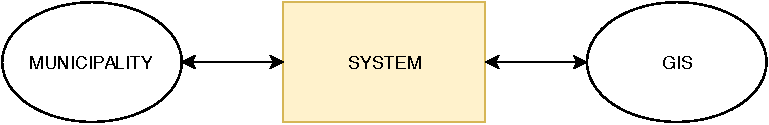
\includegraphics[scale=0.5]{system_blocks}
			\caption{
				\label{fig:systemInterfaces} 
				Overview of system interfaces
			}
		\end{figure}
	\paragraph{Mobile application}
	When a user notices a violation can interact with the system  through the mobile application. The user can upload pictures, the type of the violation and the position in which it occurred.
	
	\paragraph{Authorities} In order to mine the information collected by SafeStreets the system will provide for the authorities an interface. Information shared are the type of the violation, the name of the street where the violation occurred, and the mined information.

	\paragraph{Unsafe Areas} The system will interact with municipality service allows users to retrieve the information about the accidents that occur on the territory of the municipality. Our system will cross information provided by the municipality with users' to identify dangerous areas and provide possible solutions to the problems highlighted by the data. 
	
	\paragraph{Tickets} The software will also offer an interface that deals with the service offered by the municipality that generates tickets from the violations provided by SafeStreets. The data shared will be type of information and the plate of the car that made the violation. Integrity of the information will be ensured by the system.
	
\subsection{User Characteristics}
	We make a distinction between normal users and authorities because of their different role in the system. 
	\subsubsection{User interfaces - normal user}
	The normal user is every adult that sees a violation and decides to upload a picture of it.
	Using the interfaces of the system users can:
	\begin{enumerate}
		\item Register and log-in to the system
		\item Upload a picture of the violation with all the possible metadata
		\item Retrieve information about accidents and statistics about dangerous areas
		\item View and edit personal information
	\end{enumerate}
	
	\subsubsection{User interfaces - authority}
		An authority is a legally recognised police force or state institution.
		Using the interfaces of the system authorities can:
		\begin{enumerate}
			\item Log-in to the system with the account provided by SafeStreet, or request an account
			\item Mine the information received by the system
			\item Retrieve information about accidents and statistics about dangerous areas
			\item View information stored by SafeStreets
		\end{enumerate}
	
\subsubsection{Software interfaces}
Databases and DBMSs are clearly required in order to store data about users, plates, violations, safe/unsafe areas etc.

As mentioned before (see \hyperref[sec:systemInterfaces]{system interfaces section}) the system needs to use external APIs and to expose interfaces in order to interact with other systems.

All vehicles have an embedded external software system, which is able to display all information described in \hyperref[sec:cars]{cars section}.

\subsection{User characteristics}
	Users can use our system when they want to rent a car.\\
	Necessary conditions for the user in order to use the system are:
	\begin{itemize}
		\item He must have a smartphone and be able to use it
		\item He must be in the age of majority
		\item He must have a proper valid driving license
		\item He must be able to drive a car (i.d. he must be in both physical and mental health)
	\end{itemize}
	The user agrees to these conditions during the registration to the system.

\subsection{Domain assumption}
	We assume that these assumptions hold true in the domain of our system 
	\begin{enumerate}[label=\textbf{DA\arabic*}]
		\item GPS position is supposed to be accurate (max error $\pm5$m)
		\item GPS position of all users is always obtainable
		\item Internet connection always works correctly
		\item Municipality services are always reachable
		\item Charging station can exclusively be used by PowerEnJoy cars
		\item The set of safe areas is pre-defined and is provided to our system by the customer
		\item The maps provided by the GIS are always up to date
		
	\end{enumerate}
	
\clearpage
\subsection{The World and the Machine}
The world and the machine is a way of thinking about problems and phenomena relevant in the reality of the software system we are to develop. The world contains the phenomena that happens in reality but are not observable by our system; the machine instead contains the phenomena which take place inside the system and are not observable from outside of it. The intersection between these two sets of phenomena is the so called set of shared phenomena, which contains the phenomena that are controlled by the world and observed by the machine or controlled by the machine and observed by the world.
\newline
\\
Goals are prescriptive assertions formulated in terms of world phenomena (not necessarily shared); domain properties/assumptions are descriptive assertions assumed to hold in the world; requirements are prescriptive assertions formulated in terms of shared phenomena.\cite{WorldMachine}
\\
\\

\begin{figure}[h!]
	\centering
	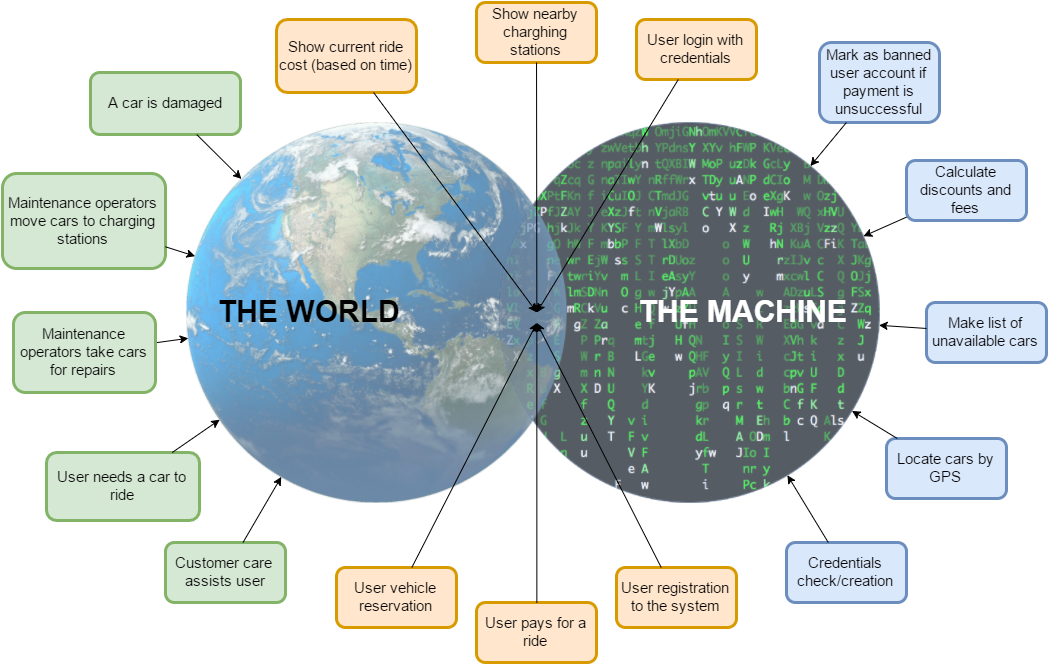
\includegraphics [width=\textwidth]{TheWorldAndTheMachine}
	\caption{
		\label{fig:WorldandMachine} 
		The World and the Machine
	}
\end{figure}
\clearpage